\section{Amazon QuickSight}

Amazon QuickSight \cite{aws-quicksight} es una herramienta de inteligencia de negocio
basada en la nube capaz de escalar si así lo requiere, además que podemos combinar data de diferentes
orígenes.

Cuando tú tienes la correcta información en el momento correcto puedes tomar mejores decisiones.

Algunos de los beneficios: \
\begin{description}
	\item[In Memory Engine:] Guarda la data en memoria haciendo más rápida las consultas posteriores
	\item[Collaborative:] No hay necesidad de instalar alguna aplicación
	\item[Publish and Share:] Puedes compartir tus análisis como un dashboard
\end{description}

\subsection{¿Cómo trabaja?}
\begin{figure}[h!]
	\centering
	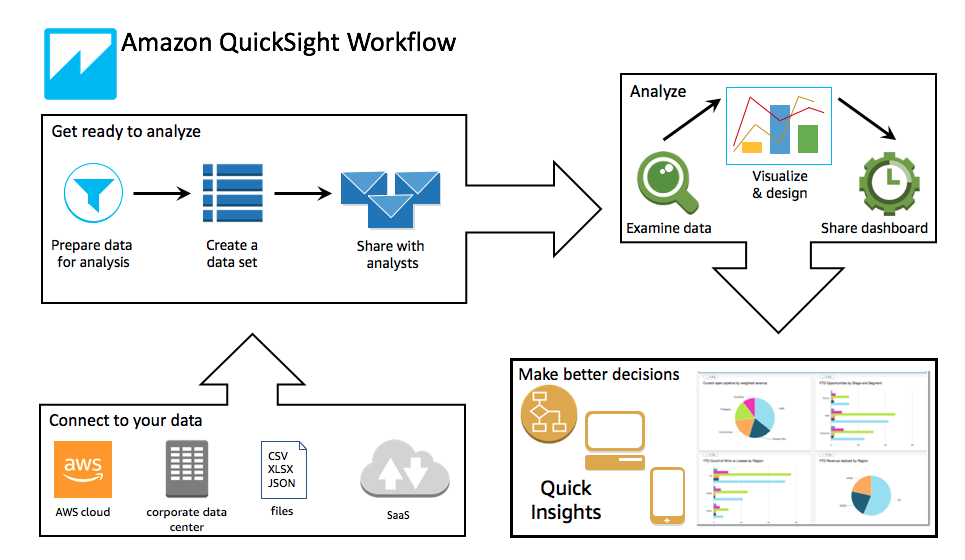
\includegraphics[width=\columnwidth]{images/aws_quicksight}
	\caption{Workflow QuickSight}
	\label{fig:quicksight_workflow}
\end{figure}

Tenemos que preparar la data para su respectivo análisis. Esto podría incluír hacer cambios en: \
\begin{itemize}
	\item Filtrar data que sea más relevante para ti
	\item Renombrar columnas para una mejor lectura
	\item Cambiar algunos tipos de datos por otros
	\item Creando una sql para refinar la data.
\end{itemize}

\subsection{Orígenes de data soportados}
Podemos usar: \
\begin{itemize}
	\item Amazon Athena
	\item Amazon Aurora
	\item Amazon Redshift
	\item Amazon S3
	\item Apache Spark
	\item Google Bigquery
	\item Mysql
\end{itemize}

\subsection{Actualizando la Data}
Hay 2 maneras: \
\begin{description}
	\item[Direct Query:] Si usas esta opción cada vez que tu ingreses al dashboard tu verás que la información está actualizada
	\item[SPICE:] No se actualiza, tienes que de forma manual, eliminar el dataset y volver a crearlo para que pueda tomar la información de nuevo.
\end{description}

\subsection{Precios y Límites}
Cuenta con los siguientes planes: \
\begin{description}
	\item[Standard Edition:] Cobro por usuarios y existe una tarifa base, ideal para pequeños equipos o empresas que necesitan crear informes o dashboards básicos
	\item[Enterprise Edition:] Cobro basado en sesiones, una sesión se considera la visita al sitio en un rago de 30 min, tarifa por usuario lector, tienes acceso a mas herramientas de ML, Active Directory
\end{description}
